\documentclass[12 pt]{article}
\usepackage{amsmath}
\usepackage{amssymb}
\usepackage{amsthm}
\usepackage{amsfonts}
\usepackage{graphicx}
\usepackage{multicol}
\usepackage[top=0.75in,bottom=0.75in,right=0.75in,left=0.75in]{geometry}
\usepackage{enumerate}
\usepackage{mathrsfs}
\usepackage[all]{xy}
\usepackage[usenames,dvipsnames,table,xcdraw]{xcolor}
\usepackage{bbm}
\usepackage{bm}
\usepackage{esvect}
\usepackage{vwcol}  
\usepackage{todonotes}
\usepackage{etoolbox}
\usepackage{wrapfig}
\usepackage{enumitem}
\usepackage{tikzpeople}
\usepackage{sidenotes}
\usepackage{imakeidx}
\usepackage{pdfpages}
\usepackage{tabularx}


%%%%%%%%%%
% For TikZ and PGFPlots
%%%%%%%%%%
\usepackage{pgfplots}
\pgfplotsset{compat=1.9}
\usetikzlibrary{arrows,shapes,positioning}
\usetikzlibrary{decorations.markings}
\usepgfplotslibrary{fillbetween}
\pgfplotsset{every axis/.append style={label style={font=\tiny},tick label style={font=\footnotesize}}}
\usetikzlibrary{angles}
\usetikzlibrary{quotes}
\usepackage{tikz-3dplot}
\usetikzlibrary{shadings}

\setlength{\parindent}{0pt}



\begin{document}
\begin{center}
\textbf{\LARGE Essential Trigonometry for Calculus}
\end{center}
\vspace{.25in}
\pagestyle{empty}


\begin{multicols}{2}


\section*{Graphs}


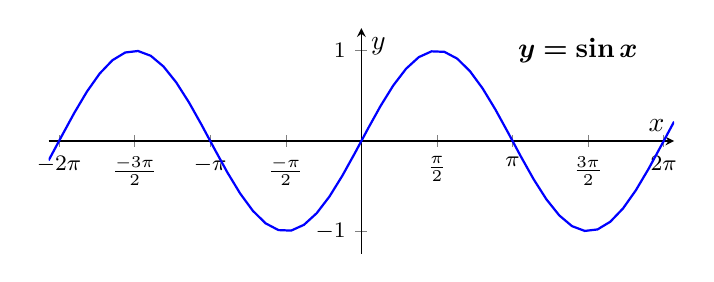
\begin{tikzpicture} 
\begin{axis}[
	width=3.75in,
	height=1.75in,
	axis lines = middle,
	xmin=-6.5, 
	xmax=6.5, 
	ymin=-1.25, 
	ymax=1.25, 
	xlabel=${x}$,
	ylabel=${y}$,
	xtick={-2*pi,-3*pi/2,-pi,-pi/2,pi/2,pi,3*pi/2,2*pi},
	ytick={-1,1},
	xticklabels = {${-2\pi}$,${\frac{-3\pi}{2}}$,${-\pi}$,${\frac{-\pi}{2}}$,${\frac{\pi}{2}}$,${\pi}$,${\frac{3\pi}{2}}$,${2\pi}$},
]
% defines the function
\addplot[  
	domain=-6.5:6.5, % the domain of the function
	blue, 
	thick,
	samples=50,
]
{sin(deg(x))};

\node at (axis cs:  4.5,1) {${\bm{y=\sin x}}$};


\end{axis}
\end{tikzpicture} 

\vfill

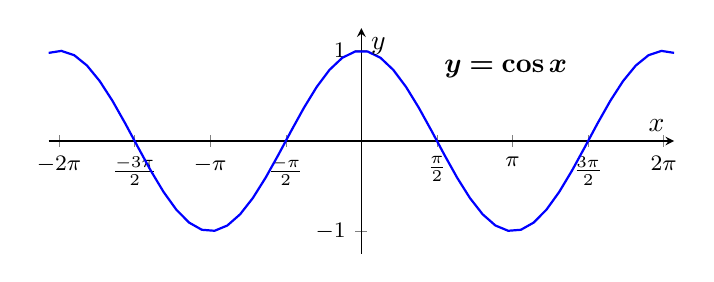
\begin{tikzpicture} 
\begin{axis}[
	width=3.75in,
	height=1.75in,
	axis lines = middle,
	xmin=-6.5, 
	xmax=6.5, 
	ymin=-1.25, 
	ymax=1.25, 
	xlabel=${x}$,
	ylabel=${y}$,
	xtick={-2*pi,-3*pi/2,-pi,-pi/2,pi/2,pi,3*pi/2,2*pi},
	ytick={-1,1},
	xticklabels = {${-2\pi}$,${\frac{-3\pi}{2}}$,${-\pi}$,${\frac{-\pi}{2}}$,${\frac{\pi}{2}}$,${\pi}$,${\frac{3\pi}{2}}$,${2\pi}$},
]
% defines the function
\addplot[  
	domain=-6.5:6.5, % the domain of the function
	blue, 
	thick,
	samples=50,
]
{cos(deg(x))};

\node at (axis cs:  3,.8) {${\bm{y=\cos x}}$};


\end{axis}
\end{tikzpicture} 
\vfill

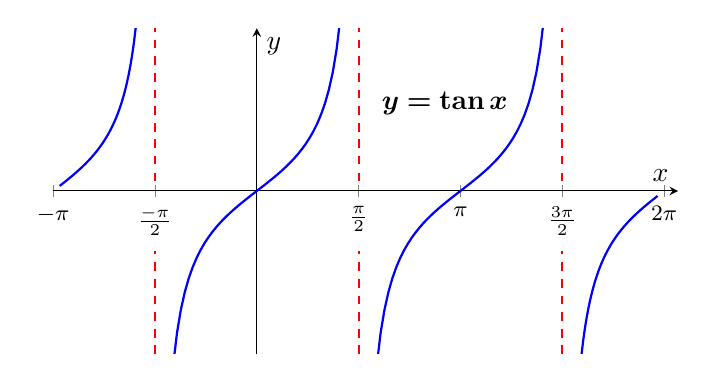
\begin{tikzpicture} 
\begin{axis}[
	width=3.75in,
	height=2.25in,
	axis lines = middle,
	xmin=-3.15, 
	xmax=6.5, 
	ymin=-3.25, 
	ymax=3.25, 
	xlabel=${x}$,
	ylabel=${y}$,
	xtick={-2*pi,-3*pi/2,-pi,-pi/2,pi/2,pi,3*pi/2,2*pi},
	ytick={-4,4},
	xticklabels = {${-2\pi}$,${\frac{-3\pi}{2}}$,${-\pi}$,${\frac{-\pi}{2}}$,${\frac{\pi}{2}}$,${\pi}$,${\frac{3\pi}{2}}$,${2\pi}$},
]
% defines the function
\addplot[  
	domain={pi/2+.1:3*pi/2-.1}, % the domain of the function
	blue, 
	thick,
	samples=50,
]
{tan(deg(x))};

\addplot[  
	domain={-pi+.1}:{-pi/2-.1}, % the domain of the function
	blue, 
	thick,
	samples=50,
]
{tan(deg(x))};

\addplot[  
	domain={3*pi/2+.1}:{2*pi-.1}, % the domain of the function
	blue, 
	thick,
	samples=50,
]
{tan(deg(x))};

\addplot[  
	domain={-pi/2+.1}:{pi/2-.1}, % the domain of the function
	blue, 
	thick,
	samples=50,
]
{tan(deg(x))};

\addplot[ % This is the parametric curve
	thick,
	dashed,
	variable=\t, % t is the parameter
	domain=-3.25:-1.2, % this is the domain of the parametric curve
    samples = 50,
    samples y=50,%prevents the starting and ending points from being joined by a line
	color=red,
]
({3*pi/2},{t});
\addplot[ % This is the parametric curve
	thick,
	dashed,
	variable=\t, % t is the parameter
	domain=-3.25:-1.2, % this is the domain of the parametric curve
    samples = 50,
    samples y=50,%prevents the starting and ending points from being joined by a line
	color=red,
]
({-pi/2},{t});


\addplot[ % This is the parametric curve
	thick,
	dashed,
	variable=\t, % t is the parameter
	domain=-3.25:-1.2, % this is the domain of the parametric curve
    samples = 50,
    samples y=50,%prevents the starting and ending points from being joined by a line
	color=red,
]
({pi/2},{t});

\addplot[ % This is the parametric curve
	thick,
	dashed,
	variable=\t, % t is the parameter
	domain=0.2:3.25, % this is the domain of the parametric curve
    samples = 50,
    samples y=50,%prevents the starting and ending points from being joined by a line
	color=red,
]
({3*pi/2},{t});
\addplot[ % This is the parametric curve
	thick,
	dashed,
	variable=\t, % t is the parameter
	domain=0.2:3.25, % this is the domain of the parametric curve
    samples = 50,
    samples y=50,%prevents the starting and ending points from being joined by a line
	color=red,
]
({-pi/2},{t});


\addplot[ % This is the parametric curve
	thick,
	dashed,
	variable=\t, % t is the parameter
	domain=0.2:3.25, % this is the domain of the parametric curve
    samples = 50,
    samples y=50,%prevents the starting and ending points from being joined by a line
	color=red,
]
({pi/2},{t});

\node at (axis cs:  2.9,1.75) {${\bm{y=\tan x}}$};


\end{axis}
\end{tikzpicture} 

\vfill


\section*{SOH--CAH--TOA}
$\displaystyle \sin\theta =\frac{\text{opposite}}{\text{hypotenuse}}$

\bigskip

$\displaystyle \cos\theta =\frac{\text{adjacent}}{\text{hypotenuse}}$

\bigskip

$\displaystyle \tan\theta =\frac{\text{opposite}}{\text{adjacent}}$

\bigskip

Popular mnemonic: ``Some Old Horse Caught Another Horse Taking Oats Away.''

\vfill
\null
\section*{Basic Identities}


\begin{multicols}{2}
$\displaystyle \tan \theta=\frac{\sin \theta}{\cos \theta}$

\bigskip

$\displaystyle\cot \theta=\frac{1}{\tan \theta}=\frac{\cos \theta}{\sin \theta}$

\bigskip

$\sin ^{2} \theta+\cos ^{2} \theta=1$

\bigskip
\vfill\null

\columnbreak
$\displaystyle\csc \theta=\frac{1}{\sin \theta}$

\bigskip

$\displaystyle\sec \theta=\frac{1}{\cos \theta}$

\bigskip

\vfill\null

\end{multicols}

\section*{Reference Triangles}

\begin{center}
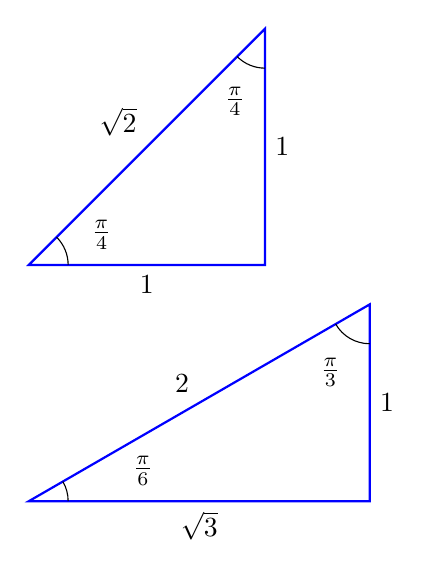
\begin{tikzpicture}

%%%%%
%% 45-45-90
%%%%%
\draw[blue, thick] (0,3) -- (3,3) node[midway,below, black] {$1$} -- (3,6) node[midway,right, black] {$1$}-- cycle node[midway,above left, black] {$\sqrt{2}$};

\coordinate (D) at (0,3);
\coordinate (E) at (3,3);
\coordinate (F) at (3,6);

\draw pic[draw,black,"{$\frac{\pi}{4}$}", angle eccentricity=2]{angle= D--F--E};
%\draw pic[draw,black]{right angle= D--E--F};
\draw pic[draw,black,"{$\frac{\pi}{4}$}", angle eccentricity=2]{angle= E--D--F};

%%%%%
%% 30-60-90
%%%%%
\draw[blue, thick]  (0,0) -- ({5*cos(30)},0) node[midway,below, black] {$\sqrt{3}$} -- ({5*cos(30)},{5*sin(30)}) node[midway,right, black] {$1$}-- cycle node[midway,above left, black] {$2$};

\coordinate (A) at (0,0);
\coordinate (B) at ({5*cos(30)},0);
\coordinate (C) at ({5*cos(30)},{5*sin(30)});


\draw pic[draw,black,"{$\frac{\pi}{3}$}", angle eccentricity=2]{angle= A--C--B};
%\draw pic[draw,black]{right angle = C--B--A};
\draw pic[draw,black,"{$\frac{\pi}{6}$}", angle eccentricity=3]{angle= B--A--C};

\end{tikzpicture}
\end{center}

\section*{Radians and Degrees}
If $d$ is the measure of an angle in degrees and $r$ is its measure in radians, then $ r=\frac{\pi}{180}d$ and $ d=\frac{180}{\pi}r$.

\begin{center}
\begin{tabular}{c c}
Degrees & Radians\\ \hline
$0^\circ$ & 0\\
$30^\circ$ & $\frac{\pi}{6}$ \\
$45^\circ$ & $\frac{\pi}{4}$\\
$60^\circ$ & $\frac{\pi}{3}$\\
$90^\circ$ & $\frac{\pi}{2}$\\
$180^\circ$ & $\pi$\\
$360^\circ$ & $2\pi$
\end{tabular}
\end{center}



\newpage
\section*{Trigonometric Identities}


$\tan ^{2} \theta+1=\sec ^{2} \theta$\\

$1+\cot ^{2} \theta=\csc ^{2} \theta$\\

$\sin (-\theta)=-\sin \theta$\\

$\cos (-\theta)=\cos \theta$\\

$\tan (-\theta)=-\tan \theta$\\

$\sin (2 \theta) =2 \sin \theta \cos \theta$\\

$\cos (2 \theta) =\cos ^{2} \theta-\sin ^{2} \theta $\\ 
\text{\,\,\,\,\,\,\,\,\,\,\,\,\,\,\,\,\,\,\,\,}$ =2 \cos ^{2} \theta-1 $\\
\text{\,\,\,\,\,\,\,\,\,\,\,\,\,\,\,\,\,\,\,\,}$=1-2 \sin ^{2} \theta $\\

$\displaystyle \tan (2 \theta) =\frac{2 \tan \theta}{1-\tan ^{2} \theta}$\\

$\sin ^{2} \theta=\frac{1}{2}(1-\cos (2 \theta)) $\\

$\cos ^{2} \theta=\frac{1}{2}(1+\cos (2 \theta)) $\\

$\displaystyle \tan ^{2} \theta=\frac{1-\cos (2 \theta)}{1+\cos (2 \theta)}$\\

$\sin \alpha \sin \beta=\frac{1}{2}(\cos (\alpha-\beta)-\cos (\alpha+\beta)) $\\

$\cos \alpha \cos \beta=\frac{1}{2}(\cos (\alpha-\beta)+\cos (\alpha+\beta)) $\\

$\sin \alpha \cos \beta=\frac{1}{2}(\sin (\alpha+\beta)+\sin (\alpha-\beta))$\\


$\sin (\alpha \pm \beta)=\sin \alpha \cos \beta \pm \cos \alpha \sin \beta$\\

$\cos (\alpha \pm \beta)=\cos \alpha \cos \beta \mp \sin \alpha \sin \beta$\\

%$\displaystyle\tan (\alpha \pm \beta)=\frac{\tan \alpha \pm \tan \beta}{1 \mp \tan \alpha \tan \beta}$\\


\begin{center}
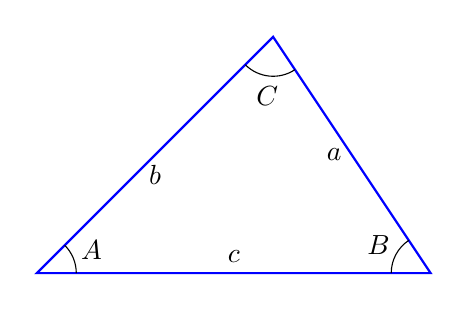
\begin{tikzpicture}

\filldraw[blue, fill=white, thick] (0,0) -- (5,0) node[midway,above, black] {$c$} -- (3,3) node[midway,left, black] {$a$}-- cycle node[midway,below, black] {$b$};

%\draw[line width=2pt,blue,-stealth](0,2)--(4,2);
%\draw[line width=2pt,red,-stealth](0,2)--(2,0) node[midway, below, sloped, black]{$\bvec{F}$};

\node(A) at (0,0) {};
%\draw [fill=black] (A) circle (2pt);
\node(B) at (5,0) {};
%\draw [fill=black] (B) circle (2pt);
\node(C) at (3,3) {};
%\draw [fill=black] (C) circle (2pt);

\draw pic[draw,black,"$C$", angle eccentricity=1.5]{angle= A--C--B};
\draw pic[draw,black,"$B$", angle eccentricity=1.5]{angle= C--B--A};
\draw pic[draw,black,"$A$", angle eccentricity=1.5]{angle= B--A--C};

\end{tikzpicture}
%\includegraphics[width=0.77\columnwidth]{triangle.pdf}\\
\end{center}

\textbf{Law of sines:} $\displaystyle\frac{\sin A}{a}=\frac{\sin B}{b}=\frac{\sin C}{c}$\\

\textbf{Law of cosines:} $c^2=a^2+b^2-2ab\cos C$

\section*{Trigonometric Limits}

$\displaystyle \lim_{x\to 0}\frac{\sin x}{x}=1$\\

$\displaystyle \lim_{x\to 0}\frac{\cos x-1}{x}=0$\\

\section*{Trigonometric Derivatives}
\noindent $\displaystyle \frac{d(\sin x)}{dx}=\cos x$\\

\noindent $\displaystyle \frac{d(\cos x)}{dx}=-\sin x$\\

\noindent $\displaystyle \frac{d(\tan x)}{dx}=\sec^2 x$\\ 

\noindent $\displaystyle \frac{d(\sec x)}{dx}=\sec x\tan x$\\

\noindent $\displaystyle \frac{d(\csc x)}{dx}=-\csc x\cot x$\\

\noindent $\displaystyle \frac{d(\cot x)}{dx}=-\csc^2 x$

\noindent $\displaystyle\frac{d}{d x}\left(\sin ^{-1} x\right) =\frac{1}{\sqrt{1-x^{2}}}$

\noindent $\displaystyle\frac{d}{d x}\left(\cos ^{-1} x\right) =-\frac{1}{\sqrt{1-x^{2}}}$

\noindent $\displaystyle\frac{d}{d x}\left(\tan ^{-1} x\right) =\frac{1}{1+x^{2}}$

\section*{Trigonometric Integrals}
\noindent $\displaystyle \int\sin x\,dx =-\cos x+C$\\

\noindent $\displaystyle \int\cos x\,dx =\sin x+C$\\

\noindent $\displaystyle \int\sec^2x\,dx =\tan x+C$\\

\noindent $\displaystyle \int\sec x\tan x\,dx =\sec x+C$\\

\noindent $\displaystyle \int\csc x\cot x\,dx =-\csc x+C$\\

\noindent $\displaystyle \int\csc^2x\,dx =-\cot x+C$\\
\end{multicols}


\newpage
\section*{The Unit Circle}
\begin{center}
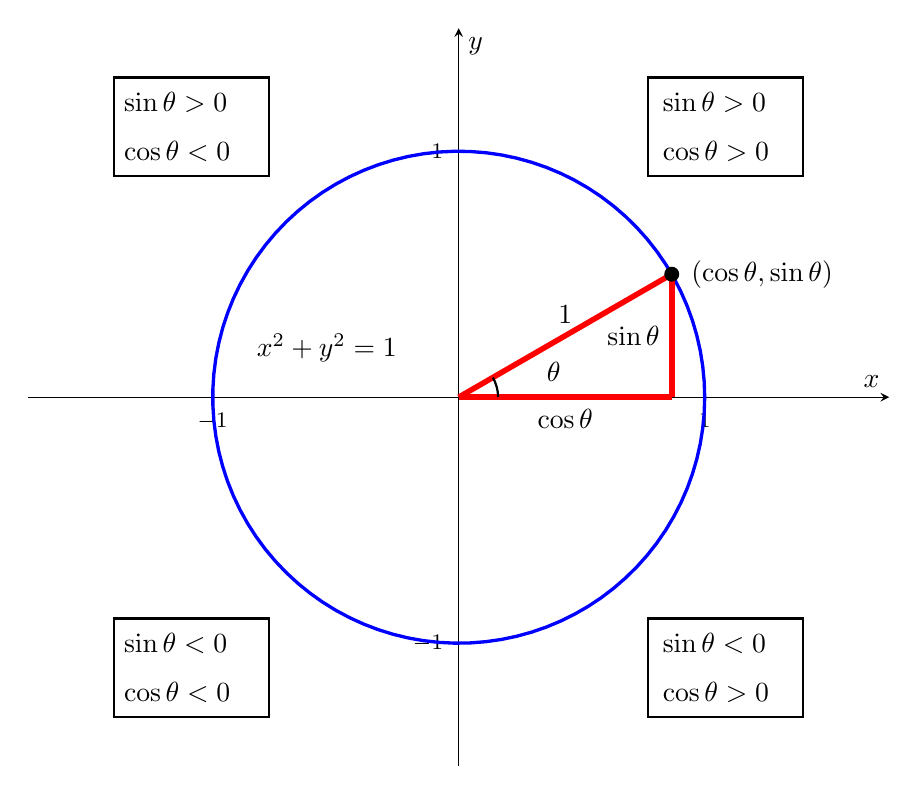
\begin{tikzpicture}
\begin{axis}[
	width=5in,
	axis lines=middle,
	xmin=-1.75,
	xmax=1.75,
	ymin=-1.5,
	ymax=1.5,
	xlabel=$x$, 
	ylabel=$y$, 
    xtick={-1,1},
    ytick={-1,1},
	unit vector ratio={1 1},
]
\addplot[ % This is the parametric curve
	very thick,
	variable=\t, % t is the parameter
	domain=0:2*pi, % this is the domain of the parametric curve
    samples = 100,
    samples y=0,%prevents the starting and ending points from being joined by a line
	color=blue,
]
({cos(deg(t))},{sin(deg(t))});

\draw[line width=2pt,red](axis cs: 0,0)--(axis cs: {cos(30)},{sin(30)}) node[midway,above,black]{$1$}; %r(t)
\draw[line width=2pt,red](axis cs: 0,0)--(axis cs: {cos(30)},0) node[midway, below, black]{$\cos  \theta$};
\draw[line width=2pt,red](axis cs: {cos(30)},0)--(axis cs: {cos(30)},{sin(30)}) node[midway, left, black]{$\sin  \theta$};

\coordinate (O) at (axis cs: 0,0);
\coordinate (A) at (axis cs: {cos(30)},{sin(30)});
\coordinate (B) at (axis cs: {cos(30)},0);

\draw pic[draw,thick,black,"$\theta$", angle eccentricity=2.5]{angle= B--O--A};
%\draw pic[draw,black]{right angle= A--B--O};

\node[label=right:${(\cos \theta,\sin \theta)}$] (E) at (axis cs: {cos(30)},{sin(30)}) {};
\draw [fill=black] (E) circle (2.5pt);

\node[label=right:${x^2+y^2=1}$] (F) at (axis cs: -.9,.2) {};

\node[label=right:${\sin\theta>0}$] at (axis cs: .75,1.2) {};
\node[label=right:${\cos\theta>0}$] at (axis cs: .75,1) {};

\node[label=right:${\sin\theta>0}$] at (axis cs: -1.44,1.2) {};
\node[label=right:${\cos\theta<0}$] at (axis cs: -1.44,1) {};


\node[label=right:${\sin\theta<0}$] at (axis cs: .75,-1) {};
\node[label=right:${\cos\theta>0}$] at (axis cs: .75,-1.2) {};

\node[label=right:${\sin\theta<0}$] at (axis cs: -1.44,-1) {};
\node[label=right:${\cos\theta<0}$] at (axis cs: -1.44,-1.2) {};


\draw[thick] (axis cs: .77,.9) -- (axis cs: .77,1.3) -- (axis cs: 1.4,1.3) -- (axis cs: 1.4,.9) -- cycle;
\draw[thick] (axis cs: -.77,.9) -- (axis cs: -.77,1.3) -- (axis cs: -1.4,1.3) -- (axis cs: -1.4,.9) -- cycle;
\draw[thick] (axis cs: -.77,-.9) -- (axis cs: -.77,-1.3) -- (axis cs: -1.4,-1.3) -- (axis cs: -1.4,-.9) -- cycle;
\draw[thick] (axis cs: .77,-.9) -- (axis cs: .77,-1.3) -- (axis cs: 1.4,-1.3) -- (axis cs: 1.4,-.9) -- cycle;

\end{axis}
\end{tikzpicture}
\resizebox{5.75in}{!}{
% Unit circle
% Author: Supreme Aryal
% A unit circle with cosine and sine values for some
% common angles.
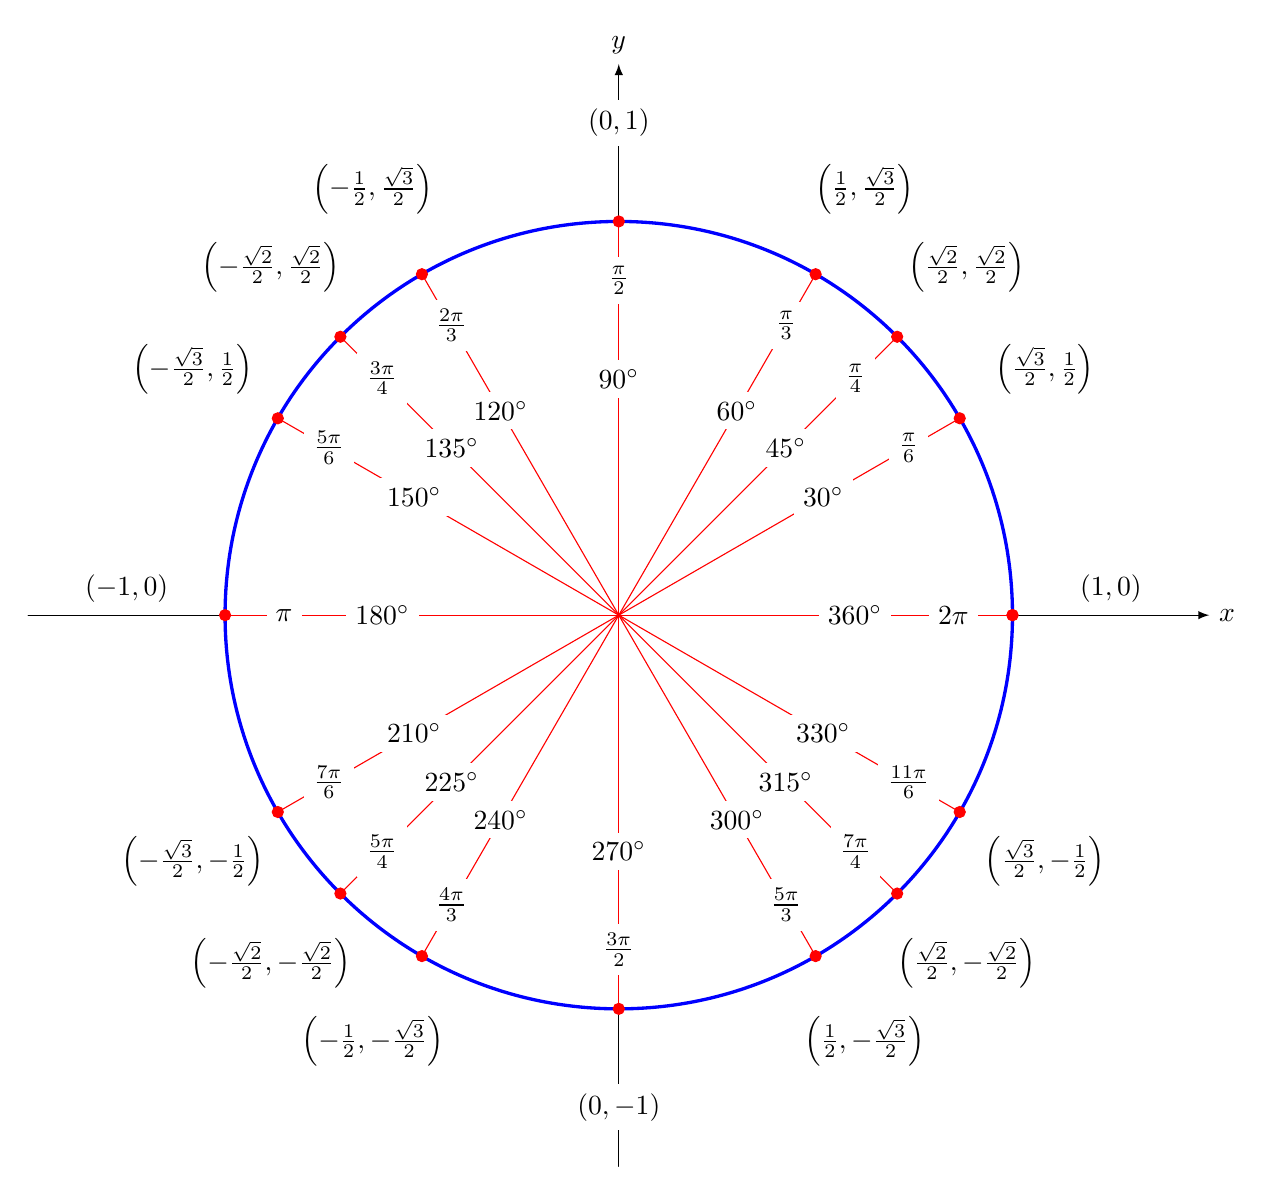
\begin{tikzpicture}[scale=5,cap=round,>=latex]
% draw the coordinates
\draw[->] (-1.5cm,0cm) -- (1.5cm,0cm) node[right,fill=white] {$x$};
\draw[->] (0cm,-1.4cm) -- (0cm,1.4cm) node[above,fill=white] {$y$};

% draw the unit circle
\draw[very thick,blue] (0cm,0cm) circle(1cm);

\foreach \x in {0,30,...,360,45,135,225,315} {
% lines from center to point
\draw[red] (0cm,0cm) -- (\x:1cm);
% dots at each point
\filldraw[red] (\x:1cm) circle(0.4pt);
% draw each angle in degrees
\draw (\x:0.6cm) node[fill=white] {$\x^\circ$};
}

% draw each angle in radians
\foreach \x/\xtext in {
30/\frac{\pi}{6},
45/\frac{\pi}{4},
60/\frac{\pi}{3},
90/\frac{\pi}{2},
120/\frac{2\pi}{3},
135/\frac{3\pi}{4},
150/\frac{5\pi}{6},
180/\pi,
210/\frac{7\pi}{6},
225/\frac{5\pi}{4},
240/\frac{4\pi}{3},
270/\frac{3\pi}{2},
300/\frac{5\pi}{3},
315/\frac{7\pi}{4},
330/\frac{11\pi}{6},
360/2\pi}
\draw (\x:0.85cm) node[fill=white] {$\xtext$};

\foreach \x/\xtext/\y in {
% the coordinates for the first quadrant
30/\frac{\sqrt{3}}{2}/\frac{1}{2},
45/\frac{\sqrt{2}}{2}/\frac{\sqrt{2}}{2},
60/\frac{1}{2}/\frac{\sqrt{3}}{2},
% the coordinates for the second quadrant
150/-\frac{\sqrt{3}}{2}/\frac{1}{2},
135/-\frac{\sqrt{2}}{2}/\frac{\sqrt{2}}{2},
120/-\frac{1}{2}/\frac{\sqrt{3}}{2},
% the coordinates for the third quadrant
210/-\frac{\sqrt{3}}{2}/-\frac{1}{2},
225/-\frac{\sqrt{2}}{2}/-\frac{\sqrt{2}}{2},
240/-\frac{1}{2}/-\frac{\sqrt{3}}{2},
% the coordinates for the fourth quadrant
330/\frac{\sqrt{3}}{2}/-\frac{1}{2},
315/\frac{\sqrt{2}}{2}/-\frac{\sqrt{2}}{2},
300/\frac{1}{2}/-\frac{\sqrt{3}}{2}}
\draw (\x:1.25cm) node[fill=white] {$\left(\xtext,\y\right)$};

% draw the horizontal and vertical coordinates
% the placement is better this way
\draw (-1.25cm,0cm) node[above=1pt] {$(-1,0)$}
  (1.25cm,0cm)  node[above=1pt] {$(1,0)$}
  (0cm,-1.25cm) node[fill=white] {$(0,-1)$}
  (0cm,1.25cm)  node[fill=white] {$(0,1)$};
\end{tikzpicture}
}
\end{center}


\end{document}


